
\documentclass[12pt,a4paper,twoside]{article}

\usepackage[margin=1in]{geometry}
\usepackage[T1]{fontenc}
\usepackage{lmodern}
\usepackage{amsmath,amssymb}
\usepackage{graphicx}
\usepackage{booktabs}
\usepackage{tabularx}
\usepackage{float}
\usepackage{caption}
\usepackage{xcolor}
\usepackage{listings}
\usepackage{pdfpages}
\usepackage{tikz}
\usetikzlibrary{positioning,arrows.meta,fit}
\usepackage{imakeidx}
\makeindex[intoc, title=Index]
\usepackage[hidelinks]{hyperref}
\usepackage{xurl}
\usepackage[toc, nonumberlist]{glossaries}
\makenoidxglossaries

\newcommand{\studentname}{Samaira Khan}
\newcommand{\entrynumber}{2024EE10201}
\newcommand{\coursecode}{ELL305}
\newcommand{\supervisor}{Prof. Subrat Kar}
\newcommand{\repourl}{\url{https://github.com/samairakhan2806/ELL305-Project-SAMAIRA-KHAN-2024EE10201/tree/main}}


\newcommand{\todo}[1]{\textcolor{red}{[#1]}}

\lstset{
  basicstyle=\ttfamily\footnotesize,
  keywordstyle=\color{blue!70!black}\bfseries,
  commentstyle=\color{green!45!black},
  stringstyle=\color{orange!70!black},
  numbers=left, numberstyle=\tiny\color{gray},
  frame=single, framerule=0.3pt, rulecolor=\color{gray!60},
  breaklines=true, columns=fullflexible, keepspaces=true,
  showstringspaces=false, tabsize=4
}


\newglossaryentry{alu}{name={ALU}, description={Arithmetic logic unit: the part of a
  processor that performs arithmetic and logical operations}}
\newglossaryentry{fpga}{name={FPGA}, description={Field-programmable gate array: a
  chip whose logic is configured after manufacture by loading a bitstream}}
\newglossaryentry{lut}{name={LUT}, description={Look-up table: the basic logic
  element of an FPGA; a LUT5 implements any Boolean function of five inputs}}
\newglossaryentry{clb}{name={CLB}, description={Configurable logic block: a group of
  LUTs and flip-flops in the FPGA fabric}}
\newglossaryentry{iob}{name={IOB}, description={Input/output block: the circuitry
  connecting an FPGA pin to the internal logic}}
\newglossaryentry{gpio}{name={GPIO}, description={General-purpose input/output: a pin
  that can be configured as an input or an output}}
\newglossaryentry{oe}{name={OE}, description={Output enable: the signal that switches
  on a pin's output driver}}
\newglossaryentry{isa}{name={ISA}, description={Instruction set architecture: the
  instructions and encodings a processor understands}}
\newglossaryentry{rv32i}{name={RV32I}, description={The 32-bit base integer
  instruction set of RISC-V}}
\newglossaryentry{spi}{name={SPI}, description={Serial Peripheral Interface: a
  synchronous serial protocol with clock, data and chip-select lines}}
\newglossaryentry{csn}{name={CS\_N}, description={Active-low chip select: frames an
  SPI transfer; its rising edge marks the end of a frame}}
\newglossaryentry{sck}{name={SCK}, description={Serial clock line of an SPI link}}
\newglossaryentry{msb}{name={MSB}, description={Most significant bit}}
\newglossaryentry{lsb}{name={LSB}, description={Least significant bit}}
\newglossaryentry{pmod}{name={PMOD}, description={A 12-pin peripheral header
  standard; on the Shrike-Lite it carries FPGA\_IO8--IO15}}
\newglossaryentry{rtl}{name={RTL}, description={Register-transfer level: a hardware
  description in terms of registers and the logic between them}}
\newglossaryentry{bitstream}{name={bitstream}, description={The configuration file
  that programs an FPGA}}
\newglossaryentry{propagate}{name={propagate}, description={In an adder, the signal
  $p_i = a_i \oplus b_i$ indicating that bit $i$ passes an incoming carry on}}
\newglossaryentry{generate}{name={generate}, description={In an adder, the signal
  $g_i = a_i \land b_i$ indicating that bit $i$ produces a carry by itself}}
\newglossaryentry{overflow}{name={overflow}, description={A signed result that does
  not fit in the available bits, e.g.\ two positive numbers giving a negative sum}}
\newglossaryentry{twoscomplement}{name={two's complement}, description={The standard
  representation of signed binary numbers, in which the negative of a number is
  formed by inverting all its bits and adding 1}}
\newglossaryentry{readability}{name={readability index}, description={A formula
  estimating the years of education needed to read a text easily}}
\glsaddall


\begin{document}


\pagenumbering{roman}
\begin{titlepage}
\centering
\vspace*{2cm}
{\LARGE\bfseries Regular versus Resource-Shared Design\\[4pt]
of an 8-bit RISC-V ALU\par}
\vspace{0.8cm}
{\large Ten Operations from One Adder and One Shifter:\\
Implementation and Hardware Verification on the Shrike-Lite FPGA\par}
\vspace{2.5cm}
{\large \studentname\\[2pt] Entry No.: \entrynumber\par}
\vspace{1cm}
{\large \coursecode\ Project Report\\[2pt] Supervisor: \supervisor\par}
\vfill
{\large Department of Electrical Engineering\\
Indian Institute of Technology Delhi\par}
\vspace{0.6cm}
{\large 13 November 2026\par}
\end{titlepage}

\setcounter{page}{2}
\section*{Copyright Assignment}
\thispagestyle{plain}

\noindent Copyright \copyright\ 2026 Indian Institute of Technology Delhi. All rights
reserved.

\medskip
\noindent I, \studentname\ (Entry No.\ \entrynumber), hereby assign all intellectual
property rights (IPR) in this report and in the work it describes, including its
text, tables, diagrams, source code, hardware designs and bitstreams, to the Indian
Institute of Technology Delhi.

\medskip
\noindent In the case of cited material, the IPR belongs to the respective authors of
the sources, as acknowledged in the References.

\vspace{2cm}
\noindent\begin{tabular}{@{}l@{}}
\rule{6cm}{0.4pt}\\
\studentname\\
Entry No.\ \entrynumber\\
Date: 13 November 2026
\end{tabular}

\clearpage
\section*{Acknowledgements}
\thispagestyle{plain}

I am thankful to Prof.\ Subrat Kar and Prof.\ Sumantra Dutta Roy, for their guidance. I am also grateful to Ms.\ Garima Singhal and to the laboratory staff, Mr.\ Utkarsh Roy and Mr.\ Deepak Priyadarshi for their help in the laboratory,
including advice on the slide-switch input and on the use of the protocol analyzer.


I gratefully acknowledge the Department of Electrical Engineering and the Indian
Institute of Technology Delhi for the use of their resources: the laboratory, the
Shrike-Lite FPGA boards, the Digilent Analog Discovery 3 analyzer and the computing
facilities.

\clearpage
\begin{abstract}
\noindent This report presents an 8-bit arithmetic logic unit (ALU) implementing the
ten integer operations of the RISC-V RV32I base instruction set (ADD, SUB, AND, OR,
XOR, SLL, SRL, SRA, SLT and SLTU), designed in Verilog and implemented on the
Vicharak Shrike-Lite board, which combines a Renesas ForgeFPGA (SLG47910V) with an
RP2040 microcontroller. Because the FPGA exposes only 14 user pins, the operands
and opcode are delivered by the RP2040 as a 24-bit SPI-style serial frame, and the
8-bit result and status flags are observed on a protocol analyzer (Digilent Analog
Discovery 3 with WaveForms). Two implementations were built: a \emph{regular} ALU
with one module per operation, and a \emph{resource-shared} ALU that realises all
ten operations with a single adder and a single shifter. Both designs were verified
on hardware against a reference model and produced identical results for every test
case, while the shared design uses 26 fewer LUTs (16.8\% of the complete design).
\end{abstract}

\clearpage
\tableofcontents
\clearpage
\listoffigures
\listoftables


\clearpage
\pagenumbering{arabic}
\section{Introduction}

The \gls{alu}\index{ALU} is the computational core of every
processor~\cite{patterson, harris}. This project implements an 8-bit ALU whose
operation set and opcode encoding follow the RISC-V\index{RISC-V} RV32I integer
instructions~\cite{riscv}.

\subsection{Relevance to ELL305}
\label{sec:relevance}

With the Table of Contents of the course textbook as reference, this project draws
upon \textbf{Chapters 1 to 12 (Instructor: Prof.\ Sumantra Dutta Roy)} of the
textbook \textbf{Basic Computer Architecture (Version 3.09)} by
Prof.\ Smruti R.\ Sarangi~\cite{sarangi} as its basis.

\subsection{Significance of the Project}
\label{sec:significance}

This project illustrates how the arithmetic logic unit, the computational core of a
processor, is built from basic digital building blocks, and how its design choices
affect the cost of the hardware. It draws together several concepts from the course
textbook. First, binary number representation: unsigned and two's complement
signed numbers, and the difference between carry, an unsigned condition, and
overflow\index{overflow}, a signed one, which the status flags make visible on the
analyzer. Second, combinational arithmetic and logic circuits: the ripple-carry
adder with its propagate and generate signals, subtraction by inverting an operand
and adding one, magnitude comparison, and logical and arithmetic shifters. Third,
instruction set architecture\index{instruction set architecture}: the ten
operations and their 4-bit opcode are taken directly from the RISC-V RV32I base
instructions, so the ALU corresponds to the execute stage of a real processor.
Fourth, sequential logic and timing: the serial loader uses a shift register, edge
detection and two-stage synchronisers on an internal clock, and the outputs are
registered so that all lines change on the same clock edge. Fifth, hardware
description and implementation: the design is written in Verilog\index{Verilog},
synthesised, placed and routed for a real FPGA, and its resource use is read from
the tool's report.

The project then extends this material. Textbooks usually present an ALU as a set
of separate function units whose outputs are selected by a multiplexer; this
structure was built as the regular design. The resource-shared design instead asks
which hardware the operations have in common. It shows that the propagate and
generate signals that every adder already computes are exactly the XOR and AND
results, that OR follows from them, that subtraction and both comparisons reuse
the same adder, and that a left shift is simply a mirrored right shift. All ten
operations therefore come from one adder and one shifter. Measured on the FPGA,
this saves 26 LUTs, or 16.8\% of the complete design, while giving identical
results on hardware. A textbook idea about sharing hardware thus becomes a
measured engineering result.

Finally, the project illustrates practical constraints that a textbook rarely
covers: a board with only 14 usable FPGA pins, which was solved with a serial input
interface, and verification on real hardware with a protocol analyzer against an
independent reference model.

\subsection{Objectives}

The objectives were:
\begin{enumerate}
  \item implement all ten RV32I register--register ALU operations at 8-bit width;
  \item fit the design onto the Shrike-Lite board;
  \item verify the design on hardware with a protocol analyzer;
  \item go beyond a textbook implementation by building a resource-shared ALU and
        quantifying its benefit.
\end{enumerate}

\section{Platform and Tools}

\begin{table}[H]
\centering
\caption{Hardware and software used.}
\label{tab:platform}
\begin{tabularx}{\linewidth}{@{}lX@{}}
\toprule
\textbf{Item} & \textbf{Details} \\
\midrule
FPGA board & Vicharak Shrike-Lite~\cite{shrike}: Renesas ForgeFPGA SLG47910V
             (Rev BB)~\cite{slg47910}, 1,120 five-input LUTs, 1,120 flip-flops,
             internal 50\,MHz oscillator, plus an RP2040
             microcontroller~\cite{rp2040}. \\
FPGA toolchain & Renesas Go Configure Software Hub (ForgeFPGA
             Workshop)~\cite{goconfigure}: synthesis, I/O planning, bitstream
             generation. \\
Microcontroller & RP2040 running Vicharak's MicroPython build~\cite{micropython},
             programmed from the Thonny IDE~\cite{thonny}; loads the bitstream
             with \texttt{shrike.flash()}. \\
Logic analyzer & Digilent Analog Discovery 3 with WaveForms~\cite{digilent}
             (Logic tool, SPI decoder). \\
\bottomrule
\end{tabularx}
\end{table}
\index{Shrike-Lite}\index{ForgeFPGA}\index{RP2040}\index{Go Configure}%
\index{Analog Discovery 3}\index{WaveForms}


\section{ALU Specification}

\subsection{Operations and opcode encoding}

The 4-bit opcode\index{opcode} is formed exactly as a RISC-V decoder would form it,
from bit 5 of the \texttt{funct7} field and the 3-bit \texttt{funct3}
field~\cite{riscv}: $\text{op} = \{\texttt{funct7}[5],\ \texttt{funct3}\}$. Shift
instructions use the low three bits of operand B as the shift amount, the 8-bit
analogue of RV32 using \texttt{rs2[4:0]} for 32-bit data. The six unused opcodes
produce a result of zero.

\begin{table}[H]
\centering
\caption{Supported operations.}
\label{tab:ops}
\begin{tabular}{@{}llll@{}}
\toprule
\textbf{Operation} & \textbf{Opcode} & \textbf{Function} & \textbf{Notes} \\
\midrule
ADD  & 0000 & $A + B$ & carry and signed overflow flags \\
SUB  & 1000 & $A - B$ & carry flag = borrow; overflow flag \\
AND  & 0111 & $A \land B$ & bitwise \\
OR   & 0110 & $A \lor B$ & bitwise \\
XOR  & 0100 & $A \oplus B$ & bitwise \\
SLL  & 0001 & $A \ll B[2{:}0]$ & logical left shift \\
SRL  & 0101 & $A \gg B[2{:}0]$ & logical right shift (zero fill) \\
SRA  & 1101 & $A \ggg B[2{:}0]$ & arithmetic right shift (sign fill) \\
SLT  & 0010 & $1$ if $A < B$ (signed) & result 00 or 01 \\
SLTU & 0011 & $1$ if $A < B$ (unsigned) & result 00 or 01 \\
\bottomrule
\end{tabular}
\end{table}

\subsection{Status flags}

RISC-V itself has no flags register; the flags\index{status flags} were added for
observability:
\begin{itemize}
  \item \textbf{Zero}: result is 00 (all operations).
  \item \textbf{Carry}: carry out of bit 7 for ADD; borrow ($A < B$ unsigned) for
        SUB; 0 otherwise.
  \item \textbf{Overflow}\index{overflow}: signed overflow for ADD and SUB;
        0 otherwise.
\end{itemize}

\section{System Architecture}

\subsection{The pin-count constraint}

A fully parallel ALU needs $8 + 8 + 4 = 20$ input pins and $8 + 3 = 11$ output
pins, 31 in total, but the Shrike-Lite exposes only 14 FPGA pins on its headers.
The design therefore receives its inputs serially: the RP2040 sends the opcode and
both operands as one 24-bit frame over three wires, leaving the FPGA pins free for
the result and flags.

\subsection{Serial input frame}

The frame\index{serial frame} uses \gls{spi}\index{SPI} mode 0 (clock idles low,
data sampled on the rising edge), MSB first, with an active-low chip select. A
rising edge on \texttt{CS\_N} marks the end of the frame and loads the operands.

\begin{table}[H]
\centering
\caption{24-bit input frame (sent MSB first).}
\label{tab:frame}
\begin{tabular}{@{}cccc@{}}
\toprule
\textbf{Bits 23--20} & \textbf{Bits 19--16} & \textbf{Bits 15--8} & \textbf{Bits 7--0} \\
\midrule
0000 & opcode & operand A & operand B \\
\bottomrule
\end{tabular}
\end{table}

\subsection{Block diagram}

\begin{figure}[H]
\centering
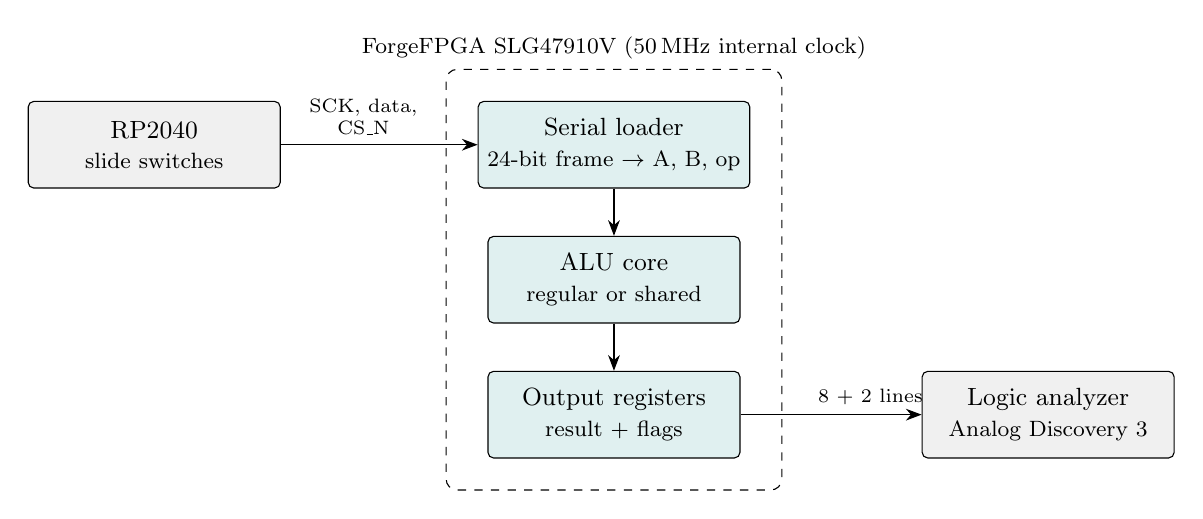
\begin{tikzpicture}[
  node distance=6mm and 10mm,
  blk/.style={draw, rounded corners=2pt, minimum width=32mm, minimum height=11mm,
              align=center, font=\small},
  ext/.style={blk, fill=gray!12},
  fpga/.style={blk, fill=teal!12},
  >={Stealth[length=2mm]}
]
\node[ext]  (rp)   {RP2040\\\footnotesize slide switches};
\node[fpga, right=25mm of rp] (rx) {Serial loader\\\footnotesize 24-bit frame $\to$ A, B, op};
\node[fpga, below=of rx] (alu) {ALU core\\\footnotesize regular or shared};
\node[fpga, below=of alu] (reg) {Output registers\\\footnotesize result + flags};
\node[ext,  right=23mm of reg] (la) {Logic analyzer\\\footnotesize Analog Discovery 3};
\node[draw, dashed, rounded corners=4pt, inner sep=4mm, fit=(rx)(alu)(reg),
      label={[font=\footnotesize]above:ForgeFPGA SLG47910V (50\,MHz internal clock)}] {};
\draw[->] (rp) -- node[above, font=\scriptsize, align=center, xshift=-2mm]{SCK, data,\\CS\_N} (rx);
\draw[->] (rx) -- (alu);
\draw[->] (alu) -- (reg);
\draw[->] (reg) -- node[above, font=\scriptsize, xshift=5mm]{8 + 2 lines} (la);
\end{tikzpicture}
\caption{System architecture. The analyzer also monitors the three input wires,
so its SPI decoder shows each frame alongside the result.}
\label{fig:block}
\end{figure}

\subsection{FPGA modules}

\begin{description}
  \item[Serial loader.]\index{serial loader} Samples SCK, data and CS\_N on the
  internal 50\,MHz clock through two-stage synchronisers, shifts one bit per
  detected rising SCK edge while CS\_N is low, and loads A, B and the opcode on the
  rising edge of CS\_N. SCK is never used as a clock, which avoids clock-domain
  problems on the FPGA.
  \item[ALU core.] Purely combinational; two interchangeable versions are
  described in Sections~\ref{sec:regular} and~\ref{sec:shared}.
  \item[Output registers.] Register the result and flags on one clock edge so that
  all output lines change simultaneously, giving clean transitions on the analyzer.
\end{description}

ForgeFPGA output pads require an explicit \gls{oe}\index{output enable} signal, so
every output port has a companion \texttt{\_oe} port driven to 1, and the internal
oscillator is enabled through a \texttt{clk\_en} port.

\subsection{Pin assignment}

Table~\ref{tab:pins} shows the final assignment\index{pin assignment}; the complete
I/O Planner settings are listed in Appendix~\ref{app:ioplanner} and the wiring in
Appendix~\ref{app:wiring}.

\begin{table}[H]
\centering
\caption{Final pin assignment.}
\label{tab:pins}
\begin{tabular}{@{}llll@{}}
\toprule
\textbf{Signal} & \textbf{FPGA pin} & \textbf{Connected to} & \textbf{Analyzer} \\
\midrule
\texttt{spi\_sck}  (in)  & FPGA\_IO18 & RP2040 GPIO14 (jumper) & DIO 11 \\
\texttt{spi\_sdi}  (in)  & FPGA\_IO7  & RP2040 GPIO17 (jumper) & DIO 12 \\
\texttt{spi\_cs\_n} (in) & FPGA\_IO0  & RP2040 GPIO16 (jumper) & DIO 13 \\
\texttt{result[7:0]}     & FPGA\_IO8--IO15 & PMOD header & DIO 0--7 \\
\texttt{zero}            & FPGA\_IO1  & header & DIO 8 \\
\texttt{carry}           & FPGA\_IO2  & header & DIO 9 \\
\texttt{overflow}        & FPGA\_IO16 & on-board LED & -- \\
\texttt{clk} / \texttt{clk\_en} & OSC\_CLK / OSC\_EN & internal oscillator & -- \\
\bottomrule
\end{tabular}
\end{table}

\section{Regular ALU}
\label{sec:regular}

The regular ALU\index{regular ALU} follows the textbook structure: each operation is
a separate module (\texttt{alu\_add}, \texttt{alu\_sub}, \texttt{alu\_and},
\texttt{alu\_or}, \texttt{alu\_xor}, \texttt{alu\_sll}, \texttt{alu\_srl},
\texttt{alu\_sra}, \texttt{alu\_slt}, \texttt{alu\_sltu}), all ten compute in
parallel, and a multiplexer driven by the opcode selects one result. This structure
is easy to read and debug, because every operation maps to exactly one module, but
it duplicates hardware that several operations could share. The source code is
listed in Appendix~\ref{app:code}.

\section{Resource-Shared ALU}
\label{sec:shared}

The shared ALU\index{resource-shared ALU} asks which hardware the ten operations
have in common. All ten are built from just two units.
Table~\ref{tab:sharing} summarises how the opcode steers them.

\begin{table}[H]
\centering
\caption{How each operation uses the two shared units (C = carry flag, V = overflow flag).}
\label{tab:sharing}
\small\begin{tabular}{@{}lllll@{}}
\toprule
\textbf{Operation} & \textbf{Unit} & \textbf{Control} & \textbf{Result taken from} & \textbf{Flags} \\
\midrule
ADD  & adder   & sub = 0 & sum $s$ & C $= c_8$, V \\
SUB  & adder   & sub = 1 & sum $s$ & C $= \lnot c_8$, V \\
SLT  & adder   & sub = 1 & $s_7 \oplus V$ & -- \\
SLTU & adder   & sub = 1 & $\lnot c_8$ (borrow) & -- \\
AND  & adder   & sub = 0 & generate $g$ & -- \\
OR   & adder   & sub = 0 & $p \lor g$ & -- \\
XOR  & adder   & sub = 0 & propagate $p$ & -- \\
SLL  & shifter & left = 1 & mirror, shift, mirror & -- \\
SRL  & shifter & arith = 0 & shift right, fill 0 & -- \\
SRA  & shifter & arith = 1 & shift right, fill sign & -- \\
\bottomrule
\end{tabular}
\end{table}

\subsection{One adder for seven operations}

An adder computes, for each bit, a \gls{propagate}\index{propagate signal} and a
\gls{generate}\index{generate signal} signal, which drive the carry
chain\index{carry chain}~\cite{harris}:
\begin{align}
  b' &= b \oplus \text{sub}, \qquad p_i = a_i \oplus b'_i, \qquad g_i = a_i \land b'_i,\\
  c_0 &= \text{sub}, \qquad c_{i+1} = g_i \lor (p_i \land c_i), \qquad
  s_i = p_i \oplus c_i .
\end{align}
These internal signals are normally hidden, but they are exactly the logic results:
\begin{itemize}
  \item XOR $= p$ and AND $= g$ (with $\text{sub}=0$), and OR $= p \lor g$;
  \item SUB uses the same adder with B inverted and carry-in 1
        (\gls{twoscomplement}\index{two's complement});
  \item SLT is the sign of $A - B$ corrected for overflow: $\text{SLT} = s_7 \oplus V$,
        where $V = c_8 \oplus c_7$;
  \item SLTU is the borrow of $A - B$: $\text{SLTU} = \lnot c_8$.
\end{itemize}

\subsection{One shifter for three shifts}

A single right shifter\index{shifter} with a selectable fill bit handles SRL
(fill 0) and SRA (fill with the sign bit). A left shift is a right shift seen in a
mirror: SLL reverses the bit order of A, shifts right, and reverses the result
back. Bit reversal\index{bit reversal} is pure wiring and costs no logic.

Worked examples for every test case are given in Appendix~\ref{app:worked}, and the
complete source code in Appendix~\ref{app:code}.

\section{Input Interface and Firmware}

\subsection{Slide-switch input}

The operands and opcode are set on 20 slide switches\index{slide switches} connected
to free RP2040 pins (Table~\ref{tab:switchpins}). Each switch connects its pin to a
shared ground bus when ON; the RP2040's internal pull-ups supply the OFF level, so
no external resistors are needed.

\begin{table}[H]
\centering
\caption{Slide-switch connections (switch ON = 1).}
\label{tab:switchpins}
\begin{tabular}{@{}lll@{}}
\toprule
\textbf{Switches} & \textbf{RP2040 pins} & \textbf{Meaning} \\
\midrule
A0--A6 & GPIO5--GPIO11 & operand A, bits 0--6 \\
A7     & GPIO15        & operand A, bit 7 \\
B0--B7 & GPIO18--GPIO25 & operand B \\
op0--op3 & GPIO26--GPIO29 & opcode \\
common & GND & ground bus \\
\bottomrule
\end{tabular}
\end{table}

\subsection{Firmware}

A MicroPython script (\texttt{alu\_test.py})\index{firmware} running on the RP2040
loads the \gls{bitstream} into the FPGA with \texttt{shrike.flash()}, reads the
switches, and sends a new 24-bit frame whenever their setting changes, after
checking that the reading has been stable for 20\,ms (which also absorbs contact
bounce). For every frame it prints the value predicted by an independent Python
reference model\index{reference model}. The RP2040 does not read the FPGA's result
back: verification consists of comparing this prediction with the result captured
by the analyzer.

\begin{lstlisting}[language=Python, caption={Frame transmission in \texttt{alu\_test.py}.}, label={lst:send}]
def send(op, a, b):
    frame = ((op & 0xF) << 16) | ((a & 0xFF) << 8) | (b & 0xFF)
    CS_N(0); time.sleep_us(10)
    for i in range(23, -1, -1):          # MSB first, SPI mode 0
        SDI((frame >> i) & 1); time.sleep_us(5)
        SCK(1); time.sleep_us(5)
        SCK(0)
    time.sleep_us(10); CS_N(1)           # rising edge -> FPGA loads A, B, op
\end{lstlisting}

\section{Tests Performed}

\subsection{Test cases}

Table~\ref{tab:vectors} lists the tests\index{test cases} performed on hardware and
the expected analyzer readings. The operands target edge cases: signed overflow, a
borrow, the difference between logical and arithmetic shifts, and signed versus
unsigned comparison.

\begin{table}[H]
\centering
\caption{Test cases and expected results.}
\label{tab:vectors}
\begin{tabular}{@{}lccccc@{}}
\toprule
\textbf{Operation} & \textbf{SPI bytes} & \textbf{Result} & \textbf{Zero} &
\textbf{Carry} & \textbf{Overflow (LED)} \\
\midrule
ADD 7F, 01  & 00 7F 01 & 80 & 0 & 0 & 1 \\
SUB 10, 20  & 08 10 20 & F0 & 0 & 1 & 0 \\
AND F0, 3C  & 07 F0 3C & 30 & 0 & 0 & 0 \\
OR F0, 0F   & 06 F0 0F & FF & 0 & 0 & 0 \\
XOR AA, FF  & 04 AA FF & 55 & 0 & 0 & 0 \\
SLL 81, 03  & 01 81 03 & 08 & 0 & 0 & 0 \\
SRL 81, 03  & 05 81 03 & 10 & 0 & 0 & 0 \\
SRA 81, 03  & 0D 81 03 & F0 & 0 & 0 & 0 \\
SLT FF, 01  & 02 FF 01 & 01 & 0 & 0 & 0 \\
SLTU FF, 01 & 03 FF 01 & 00 & 1 & 0 & 0 \\
SLL 0D, 02  & 01 0D 02 & 34 & 0 & 0 & 0 \\
\bottomrule
\end{tabular}
\end{table}

\subsection{Analyzer setup}

In WaveForms' Logic tool, DIO\,0--7 were grouped as a hexadecimal bus, DIO\,8 and
DIO\,9 shown as the zero and carry flags, and an SPI decoder configured on DIO\,11
(clock), DIO\,12 (data) and DIO\,13 (select, active low), sampling on the rising
edge, 8 bits, MSB first. The trigger was set to the falling edge of DIO\,13 (start
of frame). The full settings are listed in Appendix~\ref{app:waveforms}.

\subsection{Results of the eleven test cases}

All eleven tests produced the expected results on the analyzer, with the overflow
LED lighting only for ADD\,7F,\,01. Out of these eleven tests, the carry flag was
high only for SUB\,10,\,20 and the zero flag only for SLTU\,FF,\,01, as expected.

\subsection{Regular versus shared ALU on hardware}

Both bitstreams were loaded in turn with identical wiring and test sequence; the
analyzer showed identical results for all eleven test cases.


\section{Resource Utilisation}

Both designs were synthesised and implemented in Go Configure with identical
interface logic, pin assignment and clocking; only the ALU core differs.
Table~\ref{tab:resources} lists the figures from the Resources
Report\index{resource utilisation}.

\begin{table}[H]
\centering
\caption{Resource comparison from the Go Configure Resources Report (full design).}
\label{tab:resources}
\begin{tabular}{@{}lccc@{}}
\toprule
\textbf{Resource} & \textbf{Regular} & \textbf{Shared} & \textbf{Change} \\
\midrule
CLB LUT5s (of 1,120) & 155 (13.84\%) & 129 (11.52\%) & $-26$ ($-16.8\%$) \\
CLBs (of 140)        & 30 (21.43\%)  & 27 (19.29\%)  & $-3$ ($-10\%$) \\
Flip-flops           & 60            & 60            & unchanged \\
\quad CLB FFs        & 46            & 46            & unchanged \\
\quad IOB FFs        & 14            & 14            & unchanged \\
GPIOs (of 19)        & 14            & 14            & unchanged \\
OSCs                 & 1             & 1             & unchanged \\
\bottomrule
\end{tabular}
\end{table}

Sharing one adder and one shifter removes 26 \glspl{lut}\index{LUT}, 16.8\% of the
complete design. Because the serial loader, output registers and pin logic are
identical in both designs, the whole saving comes from the ALU core, so the
reduction within the core itself is larger than 16.8\%. The flip-flop count is
unchanged, as expected: the ALU core is purely combinational, and the change affects
only combinational logic.


\section{Conclusion}

An 8-bit ALU implementing all ten RV32I integer operations was designed,
implemented on the Shrike-Lite board and verified on hardware. A serial input
interface solved the board's pin limitation and allowed the protocol analyzer to
display each operation's inputs alongside its result. The resource-shared ALU,
built from a single adder and a single shifter, produced results identical to the
regular design in every hardware test while using 26 fewer LUTs, 16.8\% of the
complete design, according to the Go Configure Resources Report. A slide-switch
interface allows any operation and operands to be entered and verified on the
analyzer.

\section{Proposed Evaluation Scheme}
\label{sec:evaluation}

The 18 marks for the demonstration are proposed to be distributed equally
between two parts, as shown in Table~\ref{tab:evaluation}.

\begin{table}[H]
\centering
\caption{Proposed distribution of the demonstration marks.}
\label{tab:evaluation}
\begin{tabular}{@{}clc@{}}
\toprule
\textbf{Part} & \textbf{Demonstration} & \textbf{Marks} \\
\midrule
1 & Any one of the ten operations, chosen by the student & 9 \\
2 & One operation chosen by the examiner                 & 9 \\
\midrule
  & \textbf{Total}                                       & \textbf{18} \\
\bottomrule
\end{tabular}
\end{table}

\noindent In both parts, an operation counts as demonstrated when its operands
and opcode are set on the slide switches and the result captured on the protocol
analyzer matches the expected value, together with the corresponding status
flags.

\clearpage
\begin{thebibliography}{99}
\addcontentsline{toc}{section}{References}

\bibitem{riscv}
A.~Waterman and K.~Asanovi\'c (eds.),
\emph{The RISC-V Instruction Set Manual, Volume I: Unprivileged ISA},
Document Version 20191213, RISC-V Foundation, 2019.

\bibitem{sarangi}
S.~R. Sarangi, \emph{Basic Computer Architecture}, Version 3.09.
Freely available online; print edition: White Falcon Publishing, 2021.
Available: \url{https://www.cse.iitd.ac.in/~srsarangi/archbooksoft.html}

\bibitem{patterson}
D.~A. Patterson and J.~L. Hennessy,
\emph{Computer Organization and Design RISC-V Edition: The Hardware/Software
Interface}, 2nd ed., Morgan Kaufmann, 2020.

\bibitem{harris}
S.~L. Harris and D.~M. Harris,
\emph{Digital Design and Computer Architecture: RISC-V Edition},
Morgan Kaufmann, 2021.

\bibitem{slg47910}
Renesas Electronics, \emph{SLG47910 ForgeFPGA Datasheet}.
Available: \url{https://www.renesas.com}

\bibitem{goconfigure}
Renesas Electronics, \emph{Go Configure Software Hub}.
Available: \url{https://www.renesas.com}

\bibitem{shrike}
Vicharak, \emph{Shrike: documentation and examples}.
Available: \url{https://github.com/vicharak-in/shrike}

\bibitem{rp2040}
Raspberry Pi Ltd, \emph{RP2040 Datasheet}.
Available: \url{https://datasheets.raspberrypi.com/rp2040/rp2040-datasheet.pdf}

\bibitem{micropython}
MicroPython project, \emph{MicroPython documentation}.
Available: \url{https://docs.micropython.org}

\bibitem{thonny}
Thonny, \emph{Thonny: Python IDE for beginners}.
Available: \url{https://thonny.org}

\bibitem{digilent}
Digilent, \emph{Analog Discovery 3 and WaveForms reference manuals}.
Available: \url{https://digilent.com/reference}

\bibitem{amw}
Analyze My Writing, \emph{What is a Readability Index?}
Available: \url{https://www.analyzemywriting.com/readability_indices.html}

\bibitem{textstat}
textstat contributors, \emph{textstat: Python package to calculate readability
statistics of a text object}, version 0.7.13.
Available: \url{https://github.com/textstat/textstat}

\end{thebibliography}


\clearpage
\printnoidxglossary[title=Glossary]

\clearpage
\appendix

\section{Plagiarism Report}
\label{app:plagiarism}

This report was checked for plagiarism on turnitin.com. The summary below matches
the submission made there; the full Turnitin report follows.

\begin{table}[H]
\centering
\caption{Turnitin plagiarism check.}
\label{tab:plagiarism}
\begin{tabular}{@{}ll@{}}
\toprule
\textbf{Item} & \textbf{Value} \\
\midrule
Submission ID      & trn:oid:::1:3710129477\\
Date of check      & Nov 13, 2026, 1:16 PM GMT+5:30\\
Overall similarity & 11\%\\
\bottomrule
\end{tabular}
\end{table}


\clearpage
\section{Reading Indices}
\label{app:readability}

The readability of this report was assessed with the
\glspl{readability}\index{readability indices} described by Analyze My
Writing~\cite{amw}. Each index estimates the (United States) grade level, i.e.\ the
number of years of formal education, needed to read a text without difficulty; the
lower the index, the easier the text.

\subsection{Method}

Only the running text was analysed: the abstract and the prose of Sections~1--11,
including Sections~\ref{sec:relevance} and~\ref{sec:significance}.
The front matter, tables, figures, code listings, equations, appendices and
references were excluded, since they consist mainly of symbols, numbers and code
rather than sentences. The prose was extracted into a plain-text file and analysed
with \emph{textstat} (version 0.7.13)~\cite{textstat}, an open-source Python library
implementing the standard formulas; the script used,
\texttt{readability\_textstat.py}, is available in the project repository.

\subsection{Results}

\begin{table}[H]
\centering
\caption{Reading indices of the report's running text (textstat 0.7.13).}
\label{tab:readability}
\begin{tabular}{@{}lr@{}}
\toprule
\textbf{Measure} & \textbf{Value} \\
\midrule
Sentences                    & 83 \\
Words                        & 1,740 \\
Average words per sentence   & 21.0 \\
\midrule
Gunning Fog Index            & 14.20 \\
Flesch--Kincaid Grade Level  & 11.68 \\
SMOG Index                   & 13.62 \\
Coleman--Liau Index          & 11.06 \\
Automated Readability Index  & 12.86 \\
\midrule
Average grade level          & 12.69 \\
Median grade level           & 12.86 \\
\midrule
Flesch Reading Ease (0--100, higher is easier) & 48.6 \\
\bottomrule
\end{tabular}
\end{table}

\subsection{Interpretation}

The five grade-level indices range from 11.1 to 14.2, with an average of 12.7 and a
median of 12.9. On the scale given by Analyze My Writing~\cite{amw}, this
corresponds to the ``Undergraduate'' reading level (12--16), the level of college
textbooks; values above 12 are described as a thoroughly adult level, and
technical and professional literature generally scores above 12. The Flesch
Reading Ease of 48.6 agrees, placing the text in the ``difficult'' band (30--50)
typical of university-level writing. The scores are driven mainly by unavoidable
technical vocabulary (for example \emph{synchroniser}, \emph{combinational} and
\emph{oscillator}) rather than by sentence length, since the average sentence of
21.0 words is moderate. The report is therefore at an appropriate level for its
audience of engineering students. As noted by Analyze My Writing, syllable-based
indices are estimates, so other tools may give slightly different values.

\clearpage
\section{Worked Examples of the Shared ALU}
\label{app:worked}

The following examples show how the shared adder and shifter of
Section~\ref{sec:shared} produce the result of each test case in
Table~\ref{tab:vectors}.

\paragraph{ADD 7F + 01.} With sub = 0: $p = 0111\,1110$, $g = 0000\,0001$. The
carry generated in bit 0 propagates through bits 1--6, so $s = 1000\,0000 = 80$,
$c_8 = 0$ and $c_7 = 1$, giving overflow $V = c_8 \oplus c_7 = 1$: two positive
numbers produced a negative result.

\paragraph{SUB 10 $-$ 20.} With sub = 1, B is inverted to $1101\,1111$ and
$c_0 = 1$. The adder produces $s = 1111\,0000 = \mathrm{F0}$ with $c_8 = 0$, so the
borrow (carry flag) is 1.

\paragraph{SLT and SLTU on FF, 01.} Both compute $\mathrm{FF} - 01 = \mathrm{FE}$.
Signed, $s_7 = 1$ and $V = 0$, so SLT $= 1$ ($-1 < 1$). Unsigned, $c_8 = 1$ (no
borrow), so SLTU $= 0$ ($255 \not< 1$). One subtraction answers both questions.

\paragraph{SLL 0D by 2.} Mirror: $0000\,1101 \to 1011\,0000$; shift right by 2:
$0010\,1100$; mirror back: $0011\,0100 = 34$, which equals $0\mathrm{D} \ll 2$.

\paragraph{AND F0, 3C.} With sub = 0 the adder forms
$p = 1111\,0000 \oplus 0011\,1100 = 1100\,1100$ and
$g = 1111\,0000 \land 0011\,1100 = 0011\,0000$. The AND result is taken directly
from the generate signals: $g = 30$. The carry chain is not used.

\paragraph{OR F0, 0F.} Here $p = 1111\,1111$ and $g = 0000\,0000$, because the
operands share no 1-bits. The OR result is $p \lor g = 1111\,1111 = \mathrm{FF}$.
Since $g = 0$, OR and XOR coincide for these operands.

\paragraph{XOR AA, FF.} The XOR result is the propagate signal itself:
$p = 1010\,1010 \oplus 1111\,1111 = 0101\,0101 = 55$, i.e.\ every bit of A inverted.

\paragraph{SLL 81 by 3.} Mirror: $1000\,0001 \to 1000\,0001$ (this pattern reads
the same in both directions); shift right by 3 with zero fill: $0001\,0000$;
mirror back: $0000\,1000 = 08$, which equals $81 \ll 3$ truncated to 8 bits.

\paragraph{SRL 81 by 3.} The shifter fills with 0:
$1000\,0001 \to 0001\,0000 = 10$.

\paragraph{SRA 81 by 3.} The same shifter fills with the sign bit (1):
$1000\,0001 \to 1111\,0000 = \mathrm{F0}$. Read as signed numbers, $81 = -127$ and
$\mathrm{F0} = -16$: an arithmetic right shift divides by $2^3$ and rounds towards
$-\infty$ ($-127/8 = -15.875 \to -16$), whereas SRL on the same bits gives 10.

\clearpage
\section{Source Code}
\label{app:code}

The complete sources are also available in the project repository:\\
\repourl

\subsection{Resource-shared ALU}
\begin{lstlisting}[language=Verilog, caption={Resource-shared ALU (shared adder and shifter); \texttt{/hardware/main\_shared.v} in the project repository.}]
module shared_adder (
    input  [7:0] a,
    input  [7:0] b,
    input        sub,          // 1 = compute a - b
    output [7:0] sum,
    output [7:0] p,            // propagate = a ^ b'  (b' = b, or ~b when sub)
    output [7:0] g,            // generate  = a & b'
    output       cout,         // carry out of bit 7
    output       overflow      // signed overflow
);
    wire [7:0] bx = b ^ {8{sub}};      // invert b for subtraction
    wire [8:0] c;                      // carry chain

    assign p    = a ^ bx;
    assign g    = a & bx;
    assign c[0] = sub;                 // +1 completes two's complement

    genvar i;
    generate
        for (i = 0; i < 8; i = i + 1) begin : carry_chain
            assign c[i+1] = g[i] | (p[i] & c[i]);
        end
    endgenerate

    assign sum      = p ^ c[7:0];
    assign cout     = c[8];
    assign overflow = c[8] ^ c[7];     // carry into MSB != carry out of MSB
endmodule

module shared_shifter (
    input  [7:0] a,
    input  [2:0] shamt,
    input        left,         // 1 = SLL (mirror in, mirror out)
    input        arith,        // 1 = SRA (fill with sign bit)
    output [7:0] y
);
    function [7:0] reverse8(input [7:0] x);
        integer k;
        for (k = 0; k < 8; k = k + 1) reverse8[k] = x[7-k];
    endfunction

    wire [7:0] x    = left ? reverse8(a) : a;
    wire       fill = arith & a[7];
    wire [8:0] r    = $signed({fill, x}) >>> shamt;   // 9-bit: fill bit on top

    assign y = left ? reverse8(r[7:0]) : r[7:0];
endmodule

module alu_8bit (
    input      [7:0] a,
    input      [7:0] b,
    input      [3:0] op,
    output reg [7:0] y,
    output           zero,
    output reg       carry,     // ADD: carry out, SUB: borrow, else 0
    output reg       overflow   // ADD/SUB signed overflow, else 0
);
    localparam OP_ADD  = 4'b0000, OP_SLL = 4'b0001, OP_SLT = 4'b0010,
               OP_SLTU = 4'b0011, OP_XOR = 4'b0100, OP_SRL = 4'b0101,
               OP_OR   = 4'b0110, OP_AND = 4'b0111, OP_SUB = 4'b1000,
               OP_SRA  = 4'b1101;

    // SUB, SLT and SLTU all need a - b
    wire sub = (op == OP_SUB) || (op == OP_SLT) || (op == OP_SLTU);

    wire [7:0] sum, p, g, sh;
    wire       cout, v;

    shared_adder u_add (
        .a(a), .b(b), .sub(sub),
        .sum(sum), .p(p), .g(g), .cout(cout), .overflow(v)
    );

    shared_shifter u_shift (
        .a(a), .shamt(b[2:0]),
        .left(op == OP_SLL), .arith(op == OP_SRA),
        .y(sh)
    );

    wire lt_signed   = sum[7] ^ v;     // N xor V
    wire lt_unsigned = ~cout;          // borrow

    always @(*) begin
        y        = 8'h00;
        carry    = 1'b0;
        overflow = 1'b0;
        case (op)
            OP_ADD:  begin y = sum; carry = cout;  overflow = v; end
            OP_SUB:  begin y = sum; carry = ~cout; overflow = v; end
            OP_SLT:  y = {7'b0, lt_signed};
            OP_SLTU: y = {7'b0, lt_unsigned};
            OP_XOR:  y = p;
            OP_AND:  y = g;
            OP_OR:   y = p | g;
            OP_SLL, OP_SRL, OP_SRA: y = sh;
            default: y = 8'h00;
        endcase
    end

    assign zero = (y == 8'h00);
endmodule

module serial_loader (
    input            clk,
    input            sck_pin,
    input            sdi_pin,
    input            cs_n_pin,
    output reg [7:0] a,
    output reg [7:0] b,
    output reg [3:0] op,
    output reg       load_pulse      // one clk high when a new frame arrives
);
    reg [2:0]  sck_s;
    reg [2:0]  cs_s;
    reg [1:0]  sdi_s;
    reg [23:0] shreg;

    always @(posedge clk) begin
        sck_s <= {sck_s[1:0], sck_pin};
        cs_s  <= {cs_s[1:0],  cs_n_pin};
        sdi_s <= {sdi_s[0],   sdi_pin};
        load_pulse <= 1'b0;

        // shift one bit on each SCK rising edge while CS_N is low
        if (!cs_s[1] && (sck_s[2:1] == 2'b01))
            shreg <= {shreg[22:0], sdi_s[1]};

        // CS_N rising edge = end of frame -> load operands
        if (cs_s[2:1] == 2'b01) begin
            op         <= shreg[19:16];
            a          <= shreg[15:8];
            b          <= shreg[7:0];
            load_pulse <= 1'b1;
        end
    end
endmodule

(* top *)
module alu_top (
    (* iopad_external_pin, clkbuf_inhibit *) input clk,    // internal OSC clock
    (* iopad_external_pin *) output       clk_en,          // OSC enable

    // inputs from RP2040 (SPI-style frame)
    (* iopad_external_pin *) input        spi_sck,         // FPGA_IO18
    (* iopad_external_pin *) input        spi_sdi,         // FPGA_IO7  (moved from FPGA_IO17, see README)
    (* iopad_external_pin *) input        spi_cs_n,        // FPGA_IO0

    // outputs to protocol analyzer
    (* iopad_external_pin *) output [7:0] result,          // FPGA_IO8..IO15 (PMOD)
    (* iopad_external_pin *) output [7:0] result_oe,
    (* iopad_external_pin *) output       zero,            // FPGA_IO1
    (* iopad_external_pin *) output       zero_oe,
    (* iopad_external_pin *) output       carry,           // FPGA_IO2
    (* iopad_external_pin *) output       carry_oe,
    (* iopad_external_pin *) output       overflow,        // FPGA_IO16 = on-board LED
    (* iopad_external_pin *) output       overflow_oe
);
    assign clk_en      = 1'b1;
    assign result_oe   = 8'hFF;
    assign zero_oe     = 1'b1;
    assign carry_oe    = 1'b1;
    assign overflow_oe = 1'b1;

    wire [7:0] a, b, y;
    wire [3:0] op;
    wire       load_pulse, z, c, v;

    serial_loader u_rx (
        .clk(clk), .sck_pin(spi_sck), .sdi_pin(spi_sdi), .cs_n_pin(spi_cs_n),
        .a(a), .b(b), .op(op), .load_pulse(load_pulse)
    );

    alu_8bit u_alu (
        .a(a), .b(b), .op(op),
        .y(y), .zero(z), .carry(c), .overflow(v)
    );

    // register the outputs so all 11 lines change on the same clock edge
    // (one clean transition on the analyzer instead of glitches)
    reg [7:0] result_q;
    reg       zero_q, carry_q, overflow_q;
    always @(posedge clk) begin
        result_q   <= y;
        zero_q     <= z;
        carry_q    <= c;
        overflow_q <= v;
    end
    assign result   = result_q;
    assign zero     = zero_q;
    assign carry    = carry_q;
    assign overflow = overflow_q;

endmodule
\end{lstlisting}

\subsection{Regular ALU}
\begin{lstlisting}[language=Verilog, caption={Regular ALU; \texttt{/hardware/main.v} in the project repository.}]
module alu_add (
    input  [7:0] a,
    input  [7:0] b,
    output [7:0] y,
    output       carry,      // unsigned carry out of bit 7
    output       overflow    // signed overflow
);
    wire [8:0] sum = {1'b0, a} + {1'b0, b};
    assign y        = sum[7:0];
    assign carry    = sum[8];
    assign overflow = (a[7] == b[7]) && (y[7] != a[7]);
endmodule

module alu_sub (
    input  [7:0] a,
    input  [7:0] b,
    output [7:0] y,
    output       borrow,     // 1 when a < b (unsigned)
    output       overflow    // signed overflow
);
    wire [8:0] diff = {1'b0, a} - {1'b0, b};
    assign y        = diff[7:0];
    assign borrow   = diff[8];
    assign overflow = (a[7] != b[7]) && (y[7] != a[7]);
endmodule

module alu_and (input [7:0] a, input [7:0] b, output [7:0] y);
    assign y = a & b;
endmodule

module alu_or (input [7:0] a, input [7:0] b, output [7:0] y);
    assign y = a | b;
endmodule

module alu_xor (input [7:0] a, input [7:0] b, output [7:0] y);
    assign y = a ^ b;
endmodule

module alu_sll (input [7:0] a, input [2:0] shamt, output [7:0] y);
    assign y = a << shamt;                       // logical left
endmodule

module alu_srl (input [7:0] a, input [2:0] shamt, output [7:0] y);
    assign y = a >> shamt;                       // logical right (zero fill)
endmodule

module alu_sra (input [7:0] a, input [2:0] shamt, output [7:0] y);
    assign y = $signed(a) >>> shamt;             // arithmetic right (sign fill)
endmodule

module alu_slt (input [7:0] a, input [7:0] b, output [7:0] y);
    assign y = {7'b0, ($signed(a) < $signed(b))};  // signed compare
endmodule

module alu_sltu (input [7:0] a, input [7:0] b, output [7:0] y);
    assign y = {7'b0, (a < b)};                  // unsigned compare
endmodule

module alu_8bit (
    input      [7:0] a,
    input      [7:0] b,
    input      [3:0] op,
    output reg [7:0] y,
    output           zero,
    output reg       carry,      // ADD: carry out, SUB: borrow, else 0
    output reg       overflow    // ADD/SUB signed overflow, else 0
);
    localparam OP_ADD  = 4'b0000, OP_SLL = 4'b0001, OP_SLT = 4'b0010,
               OP_SLTU = 4'b0011, OP_XOR = 4'b0100, OP_SRL = 4'b0101,
               OP_OR   = 4'b0110, OP_AND = 4'b0111, OP_SUB = 4'b1000,
               OP_SRA  = 4'b1101;

    wire [7:0] y_add, y_sub, y_and, y_or, y_xor;
    wire [7:0] y_sll, y_srl, y_sra, y_slt, y_sltu;
    wire       c_add, v_add, c_sub, v_sub;

    alu_add  u_add  (.a(a), .b(b), .y(y_add), .carry(c_add), .overflow(v_add));
    alu_sub  u_sub  (.a(a), .b(b), .y(y_sub), .borrow(c_sub), .overflow(v_sub));
    alu_and  u_and  (.a(a), .b(b), .y(y_and));
    alu_or   u_or   (.a(a), .b(b), .y(y_or));
    alu_xor  u_xor  (.a(a), .b(b), .y(y_xor));
    alu_sll  u_sll  (.a(a), .shamt(b[2:0]), .y(y_sll));
    alu_srl  u_srl  (.a(a), .shamt(b[2:0]), .y(y_srl));
    alu_sra  u_sra  (.a(a), .shamt(b[2:0]), .y(y_sra));
    alu_slt  u_slt  (.a(a), .b(b), .y(y_slt));
    alu_sltu u_sltu (.a(a), .b(b), .y(y_sltu));

    always @(*) begin
        y        = 8'h00;
        carry    = 1'b0;
        overflow = 1'b0;
        case (op)
            OP_ADD:  begin y = y_add; carry = c_add; overflow = v_add; end
            OP_SUB:  begin y = y_sub; carry = c_sub; overflow = v_sub; end
            OP_AND:  y = y_and;
            OP_OR:   y = y_or;
            OP_XOR:  y = y_xor;
            OP_SLL:  y = y_sll;
            OP_SRL:  y = y_srl;
            OP_SRA:  y = y_sra;
            OP_SLT:  y = y_slt;
            OP_SLTU: y = y_sltu;
            default: y = 8'h00;
        endcase
    end

    assign zero = (y == 8'h00);
endmodule

module serial_loader (
    input            clk,
    input            sck_pin,
    input            sdi_pin,
    input            cs_n_pin,
    output reg [7:0] a,
    output reg [7:0] b,
    output reg [3:0] op,
    output reg       load_pulse      // one clk high when a new frame arrives
);
    reg [2:0]  sck_s;
    reg [2:0]  cs_s;
    reg [1:0]  sdi_s;
    reg [23:0] shreg;

    always @(posedge clk) begin
        sck_s <= {sck_s[1:0], sck_pin};
        cs_s  <= {cs_s[1:0],  cs_n_pin};
        sdi_s <= {sdi_s[0],   sdi_pin};
        load_pulse <= 1'b0;

        if (!cs_s[1] && (sck_s[2:1] == 2'b01))
            shreg <= {shreg[22:0], sdi_s[1]};

        if (cs_s[2:1] == 2'b01) begin
            op         <= shreg[19:16];
            a          <= shreg[15:8];
            b          <= shreg[7:0];
            load_pulse <= 1'b1;
        end
    end
endmodule

(* top *)
module alu_top (
    (* iopad_external_pin, clkbuf_inhibit *) input clk,    // internal OSC clock
    (* iopad_external_pin *) output       clk_en,          // OSC enable

    // inputs from RP2040 (SPI-style frame)
    (* iopad_external_pin *) input        spi_sck,         // FPGA_IO18
    (* iopad_external_pin *) input        spi_sdi,         // FPGA_IO7  (moved from FPGA_IO17, see README)
    (* iopad_external_pin *) input        spi_cs_n,        // FPGA_IO0

    // outputs to protocol analyzer
    (* iopad_external_pin *) output [7:0] result,          // FPGA_IO8..IO15 (PMOD)
    (* iopad_external_pin *) output [7:0] result_oe,
    (* iopad_external_pin *) output       zero,            // FPGA_IO1
    (* iopad_external_pin *) output       zero_oe,
    (* iopad_external_pin *) output       carry,           // FPGA_IO2
    (* iopad_external_pin *) output       carry_oe,
    (* iopad_external_pin *) output       overflow,        // FPGA_IO16 = on-board LED
    (* iopad_external_pin *) output       overflow_oe
);
    assign clk_en      = 1'b1;
    assign result_oe   = 8'hFF;
    assign zero_oe     = 1'b1;
    assign carry_oe    = 1'b1;
    assign overflow_oe = 1'b1;

    wire [7:0] a, b, y;
    wire [3:0] op;
    wire       load_pulse, z, c, v;

    serial_loader u_rx (
        .clk(clk), .sck_pin(spi_sck), .sdi_pin(spi_sdi), .cs_n_pin(spi_cs_n),
        .a(a), .b(b), .op(op), .load_pulse(load_pulse)
    );

    alu_8bit u_alu (
        .a(a), .b(b), .op(op),
        .y(y), .zero(z), .carry(c), .overflow(v)
    );

    reg [7:0] result_q;
    reg       zero_q, carry_q, overflow_q;
    always @(posedge clk) begin
        result_q   <= y;
        zero_q     <= z;
        carry_q    <= c;
        overflow_q <= v;
    end
    assign result   = result_q;
    assign zero     = zero_q;
    assign carry    = carry_q;
    assign overflow = overflow_q;

endmodule
\end{lstlisting}

\subsection{RP2040 firmware}
\begin{lstlisting}[language=Python, caption={RP2040 firmware; \texttt{/firmware/alu\_test.py} in the project repository.}]
import shrike, time
from machine import Pin

shrike.flash("alu.bin")
time.sleep_ms(100)

SCK  = Pin(14, Pin.OUT, value=0)
SDI  = Pin(17, Pin.OUT, value=0)
CS_N = Pin(16, Pin.OUT, value=1)

OPS = {"ADD": 0b0000, "SLL": 0b0001, "SLT": 0b0010, "SLTU": 0b0011,
       "XOR": 0b0100, "SRL": 0b0101, "OR":  0b0110, "AND":  0b0111,
       "SUB": 0b1000, "SRA": 0b1101}

def send(op, a, b):
    """Send one 24-bit frame: {0000, op} A B, MSB first, SPI mode 0."""
    frame = ((op & 0xF) << 16) | ((a & 0xFF) << 8) | (b & 0xFF)
    CS_N(0); time.sleep_us(10)
    for i in range(23, -1, -1):
        SDI((frame >> i) & 1); time.sleep_us(5)
        SCK(1); time.sleep_us(5)
        SCK(0)
    time.sleep_us(10); CS_N(1)             # rising edge -> FPGA loads A, B, op

def s8(x):                                 # 8-bit two's complement -> int
    return x - 256 if x & 0x80 else x

def expected(name, a, b):
    sh = b & 7
    r = {"ADD": a + b, "SUB": a - b, "AND": a & b, "OR": a | b, "XOR": a ^ b,
         "SLL": a << sh, "SRL": a >> sh, "SRA": s8(a) >> sh,
         "SLT": int(s8(a) < s8(b)), "SLTU": int(a < b)}[name]
    return r & 0xFF

def demo(gap_ms=500):
    """One frame per operation; trigger the analyzer on CS_N rising."""
    tests = [("ADD", 0x7F, 0x01), ("SUB", 0x10, 0x20), ("AND", 0xF0, 0x3C),
             ("OR", 0xF0, 0x0F), ("XOR", 0xAA, 0xFF), ("SLL", 0x81, 0x03),
             ("SRL", 0x81, 0x03), ("SRA", 0x81, 0x03), ("SLT", 0xFF, 0x01),
             ("SLTU", 0xFF, 0x01)]
    for name, a, b in tests:
        send(OPS[name], a, b)
        print("%-4s A=%02X B=%02X -> expect %02X" % (name, a, b, expected(name, a, b)))
        time.sleep_ms(gap_ms)

A_PINS  = [5, 6, 7, 8, 9, 10, 11, 15]      # A0..A7  (A0 = LSB)
B_PINS  = [18, 19, 20, 21, 22, 23, 24, 25] # B0..B7
OP_PINS = [26, 27, 28, 29]                 # op0..op3

SWITCH_TO_GND = True

NAMES = {v: k for k, v in OPS.items()}

def live_mode():
    pull = Pin.PULL_UP if SWITCH_TO_GND else None
    pins = [Pin(p, Pin.IN, pull) for p in A_PINS + B_PINS + OP_PINS]

    def read_all():
        v = 0
        for i, p in enumerate(pins):
            bit = p.value()
            if SWITCH_TO_GND:
                bit ^= 1                   # ON pulls the pin low -> count as 1
            v |= bit << i
        return v

    last = None
    print("Live mode: set A, B and op on the switches; the result follows.")
    while True:
        v = read_all()
        time.sleep_ms(20)
        if v == read_all() and v != last:  # same for 20 ms = settled, and changed
            last = v
            a, b, op = v & 0xFF, (v >> 8) & 0xFF, (v >> 16) & 0xF
            send(op, a, b)
            name = NAMES.get(op, "????")
            exp = ("%02X" % expected(name, a, b)) if name in OPS else "00 (unused op)"
            print("%-4s A=%02X B=%02X -> expect %s" % (name, a, b, exp))
        time.sleep_ms(10)

#while True:
#    demo()
#demo()
live_mode()
\end{lstlisting}

\clearpage
\section{I/O Planner Assignment}
\label{app:ioplanner}

Identical for both designs. Every output port is assigned to the OUT row of its
GPIO and its \texttt{\_oe} port to the OE row of the same GPIO.

\begin{table}[H]
\centering
\caption{Complete I/O Planner assignment.}
\label{tab:ioplanner-full}
\begin{tabular}{@{}lll@{}}
\toprule
\textbf{I/O Planner row} & \textbf{Port} & \textbf{Direction} \\
\midrule
OSC\_CLK          & \texttt{clk}            & input \\
OSC\_EN           & \texttt{clk\_en}        & output \\
GPIO0\_IN         & \texttt{spi\_cs\_n}     & input \\
GPIO7\_IN         & \texttt{spi\_sdi}       & input \\
GPIO18\_IN        & \texttt{spi\_sck}       & input \\
GPIO1\_OUT / \_OE & \texttt{zero} / \texttt{zero\_oe}   & output \\
GPIO2\_OUT / \_OE & \texttt{carry} / \texttt{carry\_oe} & output \\
GPIO8--GPIO15 OUT / OE & \texttt{result[0..7]} / \texttt{result\_oe[0..7]} & output \\
GPIO16\_OUT / \_OE & \texttt{overflow} / \texttt{overflow\_oe} & output \\
GPIO3--GPIO6       & -- (used for bitstream loading) & -- \\
GPIO17             & -- (unused)                     & -- \\
\bottomrule
\end{tabular}
\end{table}

\section{Wiring}
\label{app:wiring}

\begin{table}[H]
\centering
\caption{Board jumpers.}
\label{tab:jumpers}
\begin{tabular}{@{}lll@{}}
\toprule
\textbf{From} & \textbf{To} & \textbf{Signal} \\
\midrule
RP\_IO14 (left header, pin 11)  & FPGA\_IO18 (left header, pin 15) & SCK \\
RP\_IO17 (right header, pin 17) & FPGA\_IO7 (left header, pin 19)  & data \\
RP\_IO16 (right header, pin 18) & FPGA\_IO0 (left header, pin 16)  & CS\_N \\
\bottomrule
\end{tabular}
\end{table}

\begin{table}[H]
\centering
\caption{Analog Discovery 3 connections.}
\label{tab:analyzer-wiring}
\begin{tabular}{@{}lll@{}}
\toprule
\textbf{Analyzer} & \textbf{Board pin} & \textbf{Signal} \\
\midrule
GND        & board GND              & ground \\
DIO 0--7   & FPGA\_IO8--IO15 (PMOD) & result bits 0--7 \\
DIO 8      & FPGA\_IO1              & zero \\
DIO 9      & FPGA\_IO2              & carry \\
DIO 11     & FPGA\_IO18             & SCK \\
DIO 12     & FPGA\_IO7              & data \\
DIO 13     & FPGA\_IO0              & CS\_N \\
\bottomrule
\end{tabular}
\end{table}

\begin{table}[H]
\centering
\caption{PMOD header layout (column 1 at the 3.3\,V end).}
\label{tab:pmod}
\begin{tabular}{@{}lllllll@{}}
\toprule
 & \textbf{col 1} & \textbf{col 2} & \textbf{col 3} & \textbf{col 4} & \textbf{col 5} & \textbf{col 6} \\
\midrule
\textbf{top}    & 3.3\,V & GND & IO8  & IO10 & IO12 & IO14 \\
\textbf{bottom} & 3.3\,V & GND & IO9  & IO11 & IO13 & IO15 \\
\bottomrule
\end{tabular}
\end{table}

\section{WaveForms Configuration}
\label{app:waveforms}

\begin{table}[H]
\centering
\caption{Logic analyzer settings.}
\label{tab:waveforms}
\begin{tabularx}{\linewidth}{@{}lX@{}}
\toprule
\textbf{Setting} & \textbf{Value} \\
\midrule
Bus         & DIO 0--7 (DIO 0 = LSB), hexadecimal. \\
Signals     & DIO 8 (zero), DIO 9 (carry). \\
SPI decoder & Select DIO 13 (active low), Clock DIO 11, Data DIO 12; sample on
              rising edge, 8 bits, MSB first, hexadecimal. \\
Trigger     & Normal mode, falling edge of DIO 13. \\
Sample rate & 1\,MHz. \\
Time base   & about 200\,\textmu s/div for a single frame. \\
\bottomrule
\end{tabularx}
\end{table}

\clearpage
\printindex

\end{document}
